\chapter{La crisi della meccanica classica}

Il principio di equivalenza degli osservatori inerziali è rotto dalla scoperta di
Maxwell\footnote{James Clerk Maxwell (1831-1879), fisico scozzese le cui equazioni, a lui successivamente intitolate, mostrarono
la natura elettromagnetica della luce.} che la luce è un'onda elettromagnetica. Come tutte le onde fino ad allora note, 
si postulò che essa doveva propagarsi in un mezzo, detto etere.
A questo proposito Hermann Bondi scrisse\footnote{Hermann Bondi, La relatività e il senso comune, Zanichelli, pp. 36-37}:
\begin{quotation}
L'etere serviva a uno scopo, e a uno solo: rendere conto della propragazione della luce, 
essere per la luce ciò che l'aria è per il suono.
Ma l'aria può venir pesata, può venir messa in moto, può venir pompata fuori di un recipiente 
o può venir messa sotto pressione in esso; nulla di tutto ciò può essere fatto con questo 
ipotetico etere. [...]
Quindi l'etere non ha che una proprietà: aiuta a costruire una analogia tra propagazione della luce 
e propagazione del suono; [...] una falsa analogia. 
\end{quotation}

L'etere fornirebbe dunque un sistema di riferimento privilegiato, nel quale la luce si propaga 
isotropicamente con velocità $c$. In ogni altro riferimento, ad esempio nel riferimento terrestre,
la velocità della luce sarà necessariamente diversa a seconda della direzione di
propagazione. Si rese quindi necessario chiarire se l'etere fosse in moto rispetto alla Terra oppure no.

\section{Esperimento di Michelson--Morley\index{Michelson}\index{Morley}\index{esperimento!di Michelson--Morley|(}}

Se immaginiamo che l'etere sia solidale con il Sole abbiamo una evidente conseguenza: la Terra, essendo in moto 
rispetto all'etere e non trascinandolo, deve risentire di un ``vento d'etere''.
La luce quindi avrà una velocità diversa a seconda della sua direzione di moto, questo fatto può essere evidenziato 
con opportuni esperimenti che sfruttino il fenomeno dell'di interferenza. 
Michelson\footnote{Albert Abraham Michelson (1852-1931), 
primo scienziato americano a ricevere il premio Nobel (nel 1907); 
ha misurato la velocità della luce e ha inventato, sfruttando la
lunghezza d'onda della luce, un interferometro per misure precise.} e 
Morley\footnote{Edward W. Morley (1838-1923), chimico americano e collaboratore di Michelson nel
celeberrimo esperimento sull'etere.}, nel periodo 1882-1888, hanno cercato
di dedurre proprio da esperimenti di interferometria la velocità della terra
rispetto all'etere. Per fare ciò hanno creato un'apparecchiatura come quella
riportata in figura \ref{esperimentoMichelsonMorley}.

\begin{figure}[htbp]
\centering
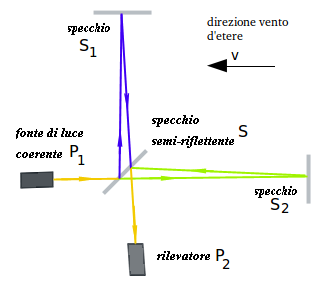
\includegraphics[scale=0.7]{immagini/michelson/Interferometro-Michelson}
\caption{\label{esperimentoMichelsonMorley}Esperimento di Michelson--Morley: Il dispositivo $P_1$ invia un fascio luminoso 
che viene parzialmente riflesso dallo specchio $S$.
Il raggio si spezza quindi in un raggio trasverso e in
un raggio longitudinale, riflessi rispettivamente dagli specchi $S_1$ e $S_2$ . I raggi
ritornano poi allo specchio $Q$ per confluire all'interfereometro $P_2$ . Dato che la
terra è in moto rispetto all'etere con una certa velocità $v$, l'interferometro $P_2$
dovrebbe rilevare frange d'interferenza.}
\end{figure}

Possiamo calcolare i tempi di percorrenza per i due diversi segnali luminosi. 
Contando che tali raggi hanno in comune il primo e l'ultimo tratto,
per il confronto ci basterà considerare il tratto trasverso (perpendicolare alla
velocità $v$, in verticale nel disegno) e il tratto longitudinale (parallelo a $v$, in
orizzontale nel disegno), entrambi di lunghezza $l$.


Nell'esperimento la luce proviene da una sorgente $P_1$, viene parzialmente riflessa da uno specchio 
semiargentato $S$ e contemporaneamente trasmessa. La luce quindi segue due cammini: $\text{I}$ e $\text{II}$; 
si riflette sugli specchi $S_1$ e $S_2$ e si riunisce in un raggio unico, prima di arrivare ad un'analizzatore. 
Le lunghezze dei percorsi dopo lo specchio $S$, $l_1$ e $l_2$ sono circa uguali, ma non uguali se riferite alla 
lunghezza d'onda della luce, quindi nell'analizzatore si dovrebbe vedere una figura d'interferenza. 
Si suppone che l'etere sia il sistema di riferimento assoluto e che l'apparecchio si muova con velocità $v$ 
verso destra, quindi si può supporre che sia l'etere a spostarsi verso sinistra con velocità $v$, il ``vento d'etere''. 
Non si considera il percorso dalla sorgente allo specchio $M$ e dallo specchio $M$ al rivelatore, in quanto i raggi viaggiano insieme. 
Il tempo per andare da $M$ a $M_1$ e tornare è:
\begin{equation}
\begin{split}
 t_1 = \frac{l_1}{c-v}+\frac{l_1}{c+v}=\frac{l_1(2c)}{c^2-v^2} = \\
    &= \frac{2c}{c^2}\frac{l_1}{1-\left(\frac{v}{c}\right)^2} = \frac{2l_1}{c}\frac{1}{1-\left(\frac{v}{c}\right)^2}
\end{split}
\end{equation}
Il percorso $\text{II}$ è ortogonale al vento d'etere, per semplicità si considera il punto di vista del vento d'etere:
\begin{figure}[htbp]
\centering
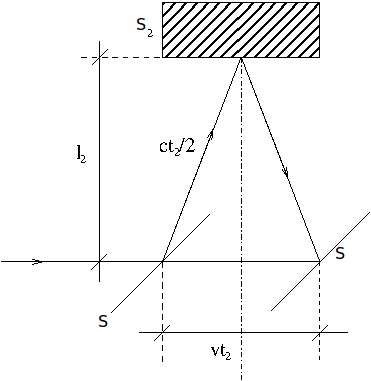
\includegraphics[scale=0.8]{immagini/michelson/Morley}
\caption{apparecchiatura vista dall'etere.}
\end{figure}

\parbox[]{\textwidth}{
\[s=2\sqrt{l_2^2+\left(\frac{vt_2}{2}\right)^2}=ct_2\]
\[l_2^2+\frac{v^2t_2^2}{4}=\frac{c^2t_2^2}{4}\qquad l_2^2=\frac{1}{4}\left(c^2-v^2\right)t_2^2\]
\[t_2=\frac{2l_2}{\sqrt{c^2-v^2}}=\frac{2l_2}{c}\frac{1}{\sqrt{1-\left(\frac{v}{c}\right)^2}}\]
}
La differenza di tempo dei due cammini è:
\[\Delta t=t_2-t_1=\frac{2}{c}\left\{\frac{l_2}{\sqrt{1-\left(\frac{v}{c}\right)^2}}-\frac{l_1}{1-\left(\frac{v}{c}\right)^2}\right\}\]
si osserva quindi una figura di interferenza. Se l'apparecchiatura viene ruotata di $90^\circ$ $l_1$ e $l_2$ si invertono:
\[\Delta t'={t_2}'-{t_1}'=\frac{2}{c}\left\{\frac{l_2}{{1-\left(\frac{v}{c}\right)^2}}-\frac{l_1}{\sqrt{1-\left(\frac{v}{c}\right)^2}}\right\}\]

\parbox[]{\textwidth}{
Si dovrebbe osservare una figura di interferenza diversa:
\begin{align*}
\Delta=&\Delta t'-\Delta t=\frac{2}{c}\left\{\frac{l_1+l_2}{{1-\left(\frac{v}{c}\right)^2}}-\frac{l_1+l_2}{\sqrt{1-\left(\frac{v}{c}\right)^2}}\right\}\\
=&\frac{2}{c}(l_1+l_2)\left\{1+\left(\frac{v}{c}\right)^2+\ldots-\left(1+\frac{1}{2}\left(\frac{v}{c}\right)^2\right)\right\}\\
\simeq&\frac{2}{c}(l_1+l_2)\frac{1}{2}\left(\frac{v}{c}\right)^2=\frac{l_1+l_2}{c}\left(\frac{v}{c}\right)^2\end{align*}
}
Con più riflessioni si riesce ad avere $l_1+l_2=\SI{20}{\metre}$, considerando il Sole come riferimento assoluto si ha $v=\SI{30}{\kilo\meter\per\second}$ e $\lambda=\SI{500E-9}{\metre}$.
Il numero di frange che scorrono dovrebbe essere:
\[\Delta N=\frac{\Delta}{T}=\frac{l_1+l_2}{\lambda}\left(\frac{v}{c}\right)^2\simeq 0.4\]
La sensibilità dello strumento era $\Delta N=0.01$. Se ci fosse stato l'etere con quella velocità sarebbe stato osservato. La ricerca dell'etere ripetuta in più mesi 
dell'anno, di giorno e di notte, usando luce solare, stellare ed artificiale, con dispositivi diversi, 
usando bracci diversi, telescopi o osservando fenomeni elettrici diede risultato negativo. 
Nel 1907 Michelson venne insignito del premio Nobel per la fisica.
\index{esperimento!di Michelson--Morley|)}

La coincidenza delle due durate può essere spiegata ripetendo formalmente i
calcoli con l'accortezza di indicare le distanze longitudinali e trasversali con
due simboli diversi (rispettivamente $l_{\parallel}$ e $l_{\bot}$). Troviamo che:
\begin{equation}
 T_{\bot} = \frac{2}{c}\dfrac{l_{\bot}}{\sqrt{1 - \frac{v^2}{c^2}}} = \frac{2}{c}\dfrac{l_{\parallel}}{1 - \frac{v^2}{c^2}} = T_{\parallel}
\end{equation}

L'esperienza di Michelson e Morley mostra che $T_{\parallel} = T_{\bot}$, e tale risultato si
spiega se ammettiamo che ovvero che $l_{\parallel} < l_{\bot}$ . Fitzgerald, nel 1892, 
concluse che il moto rispetto all'etere deve quindi comportare un fenomeno di distorsione a livello degli elettroni
(che compongono la materia, che interagiscono con forze elettromagnetiche
le quali riconoscono l'etere come osservatore privilegiato) per cui ogni regolo
si contrae nella direzione longitudinale (contrazione
delle lunghezze) della quantità:
\begin{equation}\label{gammaLorentz}
 \gamma = \dfrac{1}{\sqrt{1 - \frac{v^2}{c^2}}}
\end{equation}
la \ref{gammaLorentz} è detta fattore di Lorentz.

Se la spiegazione di Fitzgerald (che invoca un'interazione fino a quel tempo
sconosciuta tra materia ed etere responsabile del processo di contrazione)
da conto dell'esperimento nullo di Michelson e Morley, rimane aperto un secondo problema. 
L'esperimento di Michelson e Morley, infatti, è il primo
di una serie di esperimenti che mostrano che il campo elettromagnetico si
comporta nel laboratorio terrestre come previsto dalle leggi di Maxwell nell'etere. 
In sostanza, è come se le leggi di Maxwell valessero invariate in forma
sia nell'etere, sia nel laboratorio terrestre.

Nel 1895 Lorentz si pone dunque il problema di determinare matematicamente 
la più generale trasformazione di coordinate spaziotemporali che
lasci invariate in forma le equazioni di Maxwell. 

Il problema, tuttavia, era che ci si trovava di fronte ad un'incredibile coincidenza, la Terra
ritornava ad esere un sistema di riferimento privilegiato, ovvero quello in cui valgono le equazioni
di Maxwell. In un sistema di riferimento in moto rettilineo uniforme rispetto alla terra queste
equazioni diventano più complicate infatti esse non sono invarianti tra sistemi in modo. Dimostriamo questo
interessante fatto nel seguito. Per semplicità consideriamo come prototipo delle equazioni di Maxwell 
l'equazione delle onde  che in realtà è una conseguenza. 
Consideriamo il campo $E = E(x, t)$, in un universo bidimensionale. L'equazione delle onde è:
\begin{equation}
 \frac{1}{c^2} \dfrac{\partial^2 E}{\partial t^2} - \dfrac{\partial^2 E}{\partial x^2} = 0
\end{equation}

Mostriamo che tale equazione non è affatto invariante rispetto alle trasformazioni 
galileiane.

Ipotizzando infatti la trasformazione di coordinate
\begin{equation}
\left\{\begin{array}{ll}
x' = x - vt \\
t' = t
\end{array}\right.
\end{equation}

e la trasformazione della legge fisica $E (x', t') = E(x, t)$, otteniamo quindi che
$E (x - vt, t) = E(x, t)$ e dunque, calcolando le derivate parziali, si ha che:
\begin{equation}
 \left\{\begin{array}{ll}
  \dfrac{\partial E}{\partial t}(x,t) &= \dfrac{\partial E'}{\partial t'}(x-vt, t) - v \dfrac{\partial E'}{\partial x'}(x-vt,t) \\
  & \\
  \dfrac{\partial E}{\partial x}(x,t) &= \dfrac{\partial E'}{\partial x'}(x-vt, t)
 \end{array}\right.
\end{equation}

derivando nuovamente, sottintendendo i punti di calcolo delle derivate, si ha che:
\begin{equation}
 \left\{\begin{array}{ll}
  \dfrac{\partial^2 E}{\partial t^2} &= \dfrac{\partial^2 E'}{\partial t'^2} - 2v \dfrac{\partial^2 E'}{\partial x' \partial t'} + v^2  \dfrac{\partial^2 E'}{\partial x'^2} \\
  & \\
  \dfrac{\partial^2 E}{\partial x^2} &= \dfrac{\partial^2 E'}{\partial x'^2}
 \end{array}\right.
\end{equation}

Quindi, l'equazione delle onde nelle nuove coordinate assume la forma:
\begin{equation}
  \dfrac{1}{c^2}\dfrac{\partial^2 E}{\partial t'^2} - \dfrac{\partial^2 E'}{\partial x'^2} 
 - 2\dfrac{v}{c^2} \dfrac{\partial^2 E'}{\partial x' \partial t'} + \dfrac{v^2}{c^2}\dfrac{\partial^2 E'}{\partial x'^2} = 0
\end{equation}

Come si nota, tale forma è differente dalla precedente, poiché nella derivazione 
sono comparsi gli ultimi due termini che precedentemente non esistevano. 
L'equazione delle onde non è invariante in forma rispetto alle trasformazioni galileiane.